\documentclass[conference]{IEEEtran}
\IEEEoverridecommandlockouts
% The preceding line is only needed to identify funding in the first footnote. If that is unneeded, please comment it out.
\usepackage{cite}
\usepackage{amsmath,amssymb,amsfonts}
\usepackage{algorithmic}
\usepackage{graphicx}
\usepackage{textcomp}
\usepackage{xcolor}
\usepackage{subcaption}
\usepackage{kotex}
\def\BibTeX{{\rm B\kern-.05em{\sc i\kern-.025em b}\kern-.08em
    T\kern-.1667em\lower.7ex\hbox{E}\kern-.125emX}}
\begin{document}

\title{PTSD: ParTitioned Cache and request Scheduling with Demand-based FTL}

\author{\IEEEauthorblockN{Junsu Im}
\IEEEauthorblockA{\textit{ICE} \\
\textit{DGIST}\\
junsu\_im@dgist.ac.kr
}
\and
\IEEEauthorblockN{Jinwook Bae}
\IEEEauthorblockA{\textit{ICE} \\
\textit{DGIST}\\
jinwook.bae@dgist.ac.kr}
}

\maketitle

\begin{abstract}
This document is a model and instructions for \LaTeX.
This and the IEEEtran.cls file define the components of your paper [title, text, heads, etc.]. *CRITICAL: Do Not Use Symbols, Special Characters, Footnotes, 
or Math in Paper Title or Abstract.
\end{abstract}

\begin{IEEEkeywords}
component, formatting, style, styling, insert
\end{IEEEkeywords}

\section{Introduction}
This document is a model and instructions for \LaTeX.
Please observe the conference page limits. 

\section{Background And Motivation}
\subsection{NAND Flash and Address Mapping}
\begin{figure}[h]
	\centering
	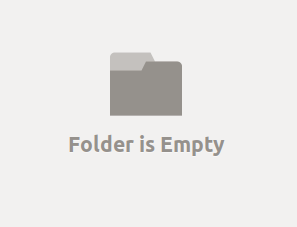
\includegraphics[width=0.2\textwidth]{image/bg.png}
	\caption{NAND Flash Chip}
	\label{fig:chips}
\end{figure}
NAND Flash의 물리적 구조는 Fig~\ref{fig:chips}과 같이 나타나 있다. NAND 칩들이 레이드 0와 비슷한 형태로 버스에 묶여져 있으며 각각의 버스는 동시에 data를 전송할 수 있는 병렬 단위가 된다. 또한 버스의 data 전송 시간 보다 칩 하나의 처리시간이 더 오래걸리기 때문에 버스에 붙여진 여러개의 칩도 병렬 단위가 된다. NAND 칩은 그 물리적 특성으로 In-place Update가 지원되지 않는다. 추가적으로 읽기와 쓰기의 단위는 하나의 물리적 페이지 단위로 이루어 질 수 있지만, 삭제 연산은 페이지의 집합인 블록 단위로 이루어진다. 이러한 두가지 기기의 특성 때문에 유저의 요청을 처리하기 위해 논리적 주소와 물리적 주소의 사상이 필요하다. \par
\begin{figure}[h]
	\centering
	\begin{subfigure}[b]{0.2\textwidth}	
		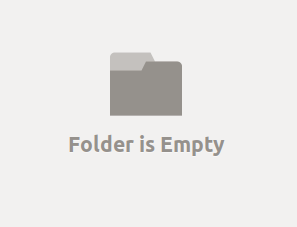
\includegraphics[width=\linewidth]{image/bg.png}
		\caption{Read/Write} \label{fig:PM}
	\end{subfigure}
	\begin{subfigure}[b]{0.2\textwidth}	
		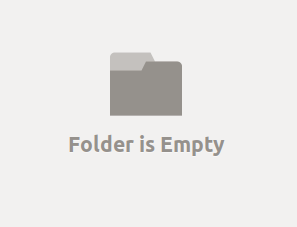
\includegraphics[width=\linewidth]{image/bg.png}
		\caption{Garbage Collection} \label{fig:GC}
	\end{subfigure}
	\caption{Page Mapping}
\end{figure}
일반적으로 성능상의 문제로 인해 사상 정보 전체를 DRAM에 저장해 두는 Page Mapping 기법을 사용한다.
DRAM 내부에는 LBA-PPA 쌍의 table이 존재하고 사용자의 요청은 이러한 사상 정보를 참고해 처리하게 된다.
PPA는 LBA와 독립적으로 존재하기 때문에 LBA에 특정한 PPA에 할당할 수 있으며 NAND Flash는 이러한 특징을 이용해 Fig~\ref{fig:chips}에서의 병렬 유닛에 맞추어 PPA를 할당하게 된다.\par
Fig~\ref{fig:PM}은 Page Mapping에서의 읽기/쓰기의 흐름을 보여준다. 들어오는 쓰기 요청은 물리적 공간에서 Logging의 형태로 적히게 되며 존재하던 정보가 새로이 들어오게 될 때 기존의 물리적 페이지가 더 이상 쓰이지 않는다는 Invalid 표시를 해두고 나중에 Garbage Collection(GC)를 통해 해당 영역을 다시 쓰게끔 동작한다.

\subsection{Garbage Collection(GC)}
GC는 더 이상 유저 쓰기 요청을 처리할 수 없을 때 발생한다. GC의 동작은 NAND의 지우기 단위인 블록의 크기로 진행되며 세가지 단계로 나누어 진다. 첫 번째로 어떠한 블록을 GC할 것인가에 대한 대상 선택의 단계이다. 이 단계에서는 Invalid 페이지가 많은 블록을 고르거나 워크로드에 맞게 Cost-benefit을 계산해 처리하는 방식이 있다. 본 논문에서는 전자의 방법을 사용하고 있다. 두 번째 단계로 Valid 페이지를 다른 블록에 Copy하는 작업이며 마지막으로는 해당 블록을 지우는 연산으로 마무리 된다.
쓰기, 읽기 연산보다 지우는 연산이 열 배 이상 걸리며 GC도중 Copy 연산이 빈번하게 일어나기 때문에 NAND 성능의 병목이 GC에서 주로 나타난다. 때문에 GC의 부하를 줄이기 위해 물리적 공간보다 적은 영역을 호스트에게 노출해 Invalid를 더 많이 분포하게 하는 over provisioning영역이 존재한다. 기본적으로 이 영역의 비율은 물리적 공간의 7\%에서 50\%까지 두게 된다.

\subsection{FTLs on limited memory environment}
\begin{figure}[h]
	\centering
	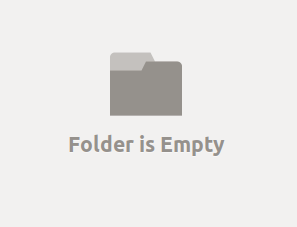
\includegraphics[width=0.2\textwidth]{image/bg.png}
	\caption{Variable Mapping Method in limited DRAM}
	\label{fig:Map}
\end{figure}
앞서 언급했듯이 본 논문은 DRAM이 제한된 환경에서의 연구를 목적으로 하고 있다. 이때까지 제시된 논문은 Fig~\ref{fig:Map}와 같이 많은 문제점이 존재한다. 블록 단위의 사상과 Hybrid사상은 읽기 연산의 경우 한 번에 접근이 가능하지만 GC연산이 빈번하게 호출되기 때문에 쓰기 연산이 많이 발생하게 되고 쓰기연산은 NAND의 수명을 줄일 뿐 아니라 많은 시간이 소모 되기 때문에 사용하기 어렵다. 반면 Demand Based사상의 경우 합리적인 읽기 쓰기 비용을 가지고 있지만 Cache의 Dirty가 eviction 문제로 인해 읽기 연산의 시간을 예상하기 힘들다.

\subsection{Demnad based FTL}

\section{PTSD}
\begin{figure}[h]
	\centering
	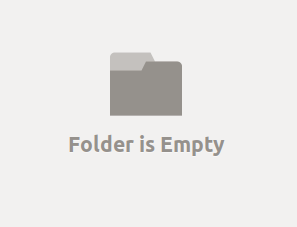
\includegraphics[width=0.2\textwidth]{image/bg.png}
	\caption{Variable Mapping Method in limited DRAM}
	\label{fig:PTSD}
\end{figure}

\subsection{Cache Partitioning}
\subsection{I/O Scheduling}
\subsection{Write Optimization}
\subsection{Future Work}

\section{Evaluation}
\subsection{Setting}
\subsection{Read CDF Trend}
\subsection{Read distribution}
\subsection{Write performance}

\section{Evaluation}

\end{document}
